%FOR PDFLATEX USE ONLY
\documentclass[a4paper,12pt]{article}

\usepackage{amssymb,amsmath} %math symbols

\usepackage[margin=2cm]{geometry} %paper geometry

\usepackage[T1, T2A]{fontenc}

\usepackage[utf8]{inputenc} %allows unicode (including russian) source file
\usepackage[russian]{babel} %docment in russian-style
\usepackage[utf8]{inputenc}
%\usepackage[unicode]{hyperref} %links inside of the text
\usepackage[pdftex]{graphicx} %includegraphics pictures
\usepackage{cmlgc} %bold text

\usepackage{array} %arrays

%\usepackage{wrapfig}
%\usepackage{array}
%\usepackage{lipsum}
%\usepackage{esvect}
%\usepackage{hyperref}

\usepackage{amsmath}
\usepackage{amssymb}
\usepackage{mathtools}
\usepackage{mathtext}

\usepackage{subfig}
%\usepackage{calc}
%\usepackage{pgfplots,tikz,circuitikz}
%\usepackage{tkz-euclide}

\begin{document}

\begin{center}
  \LARGE{Работа 3.3.4}\\[0.2cm]
  \LARGE{Эффект Холла в полупроводниках}\\[0.2cm]
  \large{Малиновский Владимир}\\[0.2cm]
  \normalsize{\texttt{galqiwi@galqiwi.ru}}
\end{center}

\textbf{Цель работы:} измерение подвижности и концентрации носителей заряда в полупроводниках\\
\textbf{В работе используются:} электромагнит с источником питания, амперметр, миллиамперметр, реостат, цифровой аольтметр, источник питания ($1.5 \text{В}$), образцы легированного германия\\
\section*{Идея}
Эффект хола заключается в возникновении разницы потенциалов на поверхности материала при протекании тока через этот материал, если этот материал помещен в магнитное поле. Собственно, в этой работе мы будем помещать образец легированного германия в магнитное поле и измерим зависимость разницы потенциалов между контактами $3-4$ от внешнего поля $B$, вызванного электромагнитами. Также, используя зависимость разницы потенциалов между точками $3-4$ от $I$, мы найдем проводимость $\sigma$, из которой вычеслим постоянную Холла.

\begin{center}
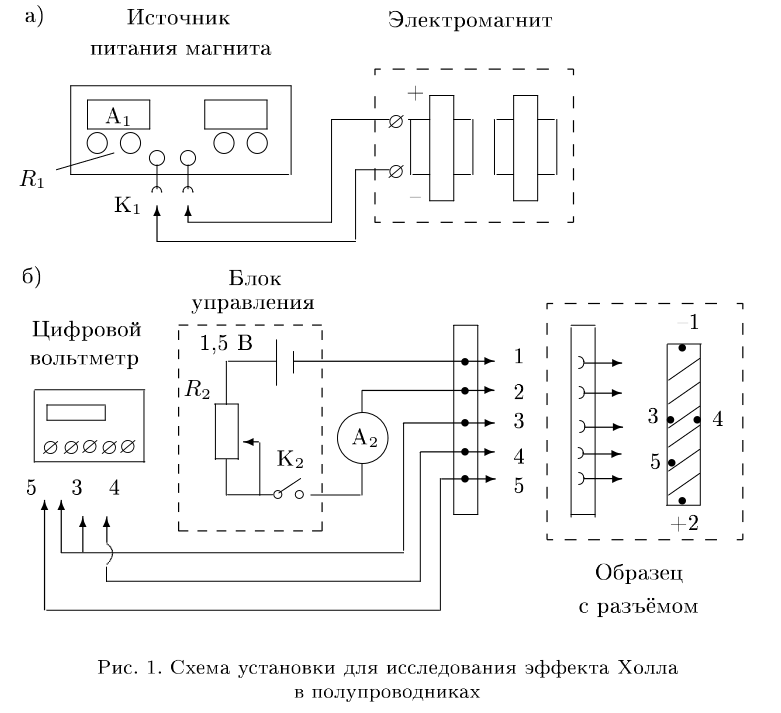
\includegraphics[width=0.80\textwidth]{setup.png}
\end{center}

\section*{Метод, результаты и обработка}
\subsection*{1-4}
Проверим работу электромагнита и прокалибруем его, измерив зависимость $\Phi$ потока через милливеберметр от тока $I_\text{м}$ через магнит. Из нее найдем поле $B = \Phi / (NS)$, идущее через милливеберметр с $NS = 75\,\text{см}^2$.

\begin{center}
\begin{tabular}{|l|l|l|l|l|l|l|l|l|}\hline
$I$, А & 0.20 & 0.40 & 0.60 & 0.80 & 1.00 & 1.20 & 1.40 & 1.60 \\ \hline
$\Phi$, мВб & 1.10 & 2.20 & 3.30 & 4.40 & 5.20 & 5.80 & 6.30 & 6.60 \\ \hline
$B$, мТл & 147 & 
293 & 440 & 587 & 693 & 773 & 840 & 880 \\ \hline
\end{tabular}\\~\\
$\Delta I=0.005\,\text{A}, \Delta \Phi=0.05\,\text{мВб}, \Delta B=13\,\text{мТл}$
\end{center}
\begin{center}
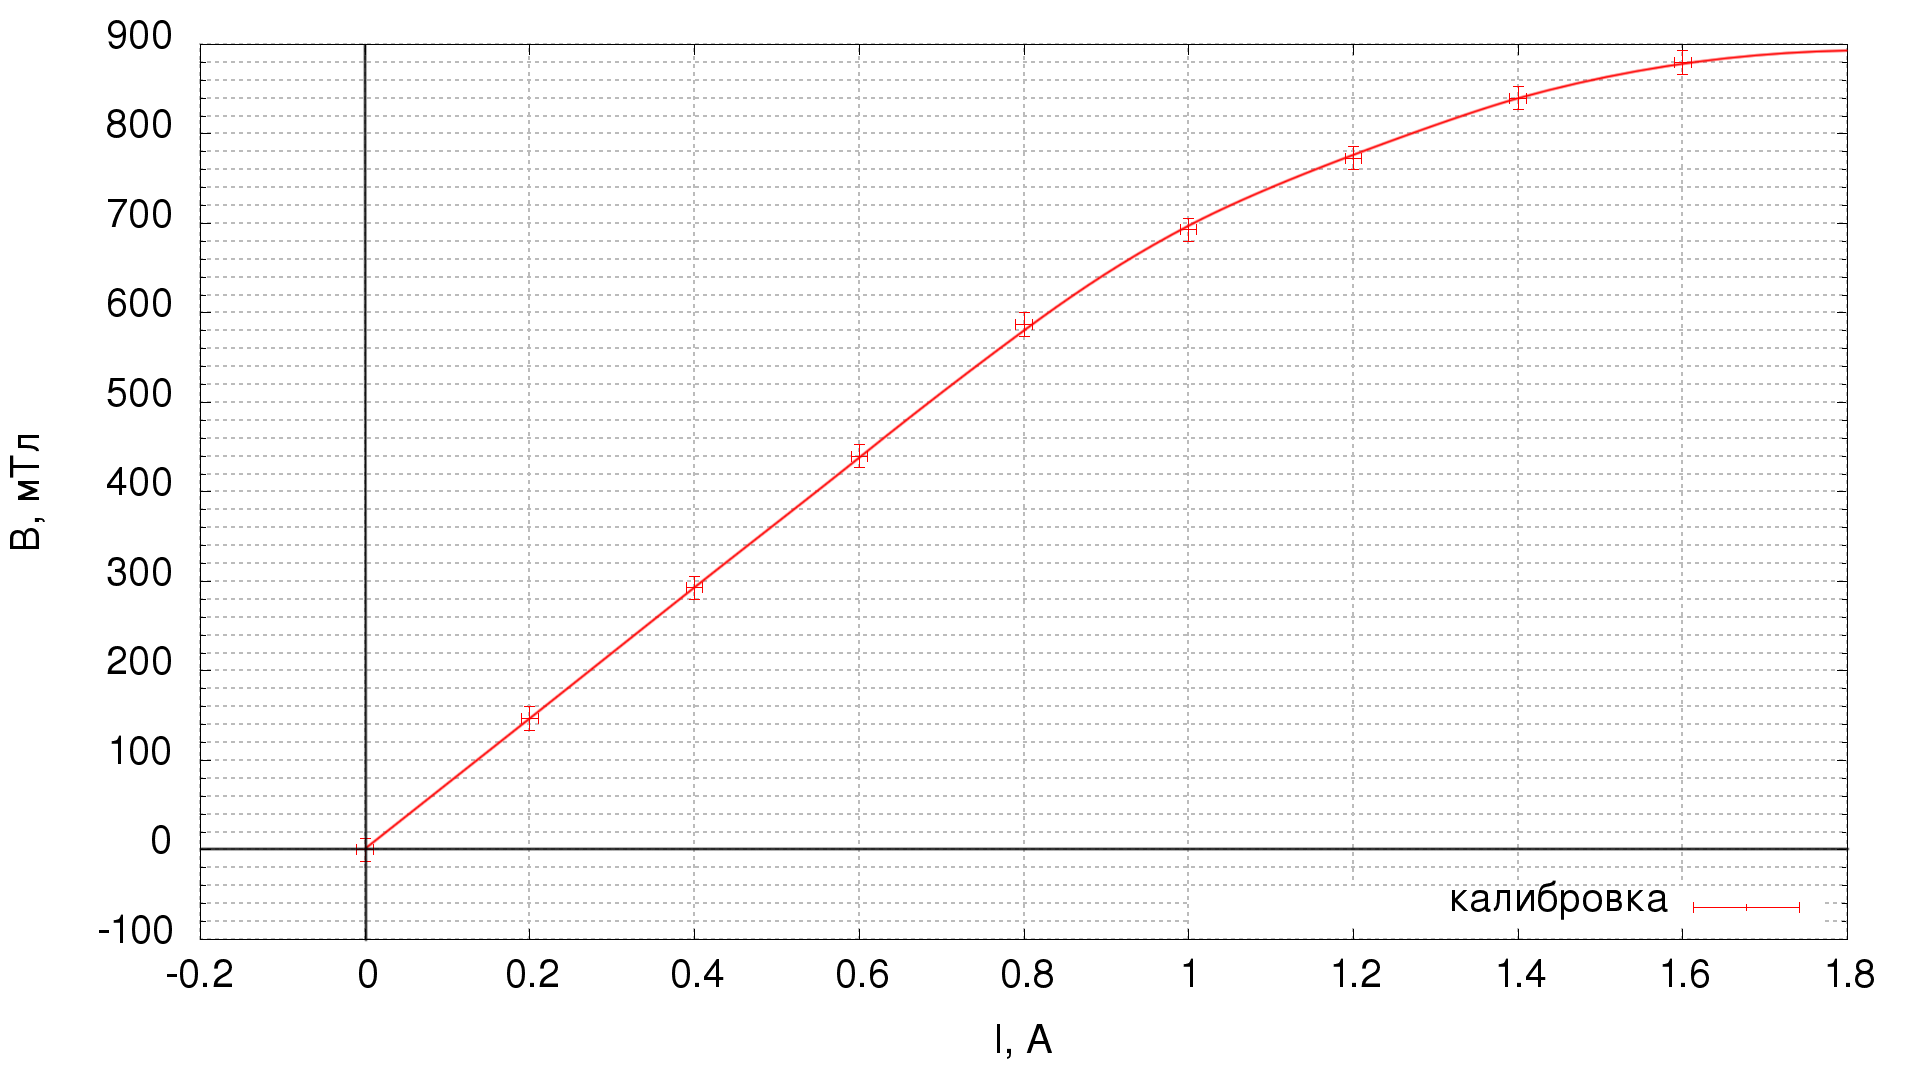
\includegraphics[width=0.80\textwidth]{calib.png}
\end{center}
\subsection*{5}
Измерим ЭДС Холла. Для фиксированного тока через образец $I$ в электромагните измерим зависимость напряжения $U_{34}$ от тока $I_M$ на электромагните.

\begin{center}
\begin{tabular}{|l|l|l|l|l|l|l|l|l|l|}
\hline
\multicolumn{10}{|l|}{$I$, мА}  \\ \hline
0.26 & 0.30 & 0.40 & 0.50 & 0.60 & 0.70 & 0.80 & 0.90 & 1.00 & -1.00 \\ \hline
\multicolumn{10}{|l|}{$U_{34}$, мкВ}  \\ \hline
40	&	46	&	63	&	78		&	93		&	109		&	125		&	141		&	157		&	172 \\ \hline
22	&	23	&	32	&	40		&	48		&	57		&	62		&	73		&	80		&	248 \\ \hline
1	&	2	&	1	&	1		&	4		&	1		&	2		&	5		&	4		&	329 \\ \hline
-16	&	-19	&	-25	&	-33		&	-39		&	-45		&	-51		&	-57		&	-65		&	405 \\ \hline
-31	&	-37	&	-50	&	-63		&	-75		&	-89		&	-103	&	-113	&	-127	&	466 \\ \hline
-45	&	-52	&	-70	&	-87		&	-104	&	-123	&	-141	&	-156	&	-175	&	520 \\ \hline
-52	&	-61	&	-82	&	-104	&	-124	&	-125	&	-165	&	-185	&	-206	&	554 \\ \hline
-58	&	-68	&	-91	&	-115	&	-137	&	-161	&	-183	&	-206	&	-228	&	580 \\ \hline
-62	&	-72	&	-96	&	-122	&	-145	&	-170	&	-193	&	-217	&	-241	&	593 \\ \hline
\end{tabular}\\[0.4cm]
$\Delta I = 0.01\,\text{мА}, \Delta U_{34} = 1\,\text{мкВ}$
\end{center}

\begin{center}
\begin{tabular}{|l|l|l|l|l|l|l|l|l|l|}
\hline
\multicolumn{10}{|l|}{$I_M$, А}  \\ \hline
0.00 & 0.00 & 0.00 & 0.00 & 0.00 & 0.00 & 0.00 & 0.00 & 0.00 & 0.00 \\ \hline
0.20 & 0.20 & 0.20 & 0.20 & 0.20 & 0.20 & 0.20 & 0.20 & 0.20 & 0.20 \\ \hline
0.40 & 0.40 & 0.40 & 0.40 & 0.40 & 0.40 & 0.40 & 0.40 & 0.40 & 0.40 \\ \hline
0.60 & 0.60 & 0.60 & 0.60 & 0.60 & 0.60 & 0.60 & 0.60 & 0.60 & 0.60 \\ \hline
0.80 & 0.80 & 0.80 & 0.80 & 0.80 & 0.80 & 0.80 & 0.80 & 0.80 & 0.80 \\ \hline
1.00 & 1.00 & 1.00 & 1.00 & 1.00 & 1.00 & 1.00 & 1.00 & 1.00 & 1.00 \\ \hline
1.20 & 1.20 & 1.20 & 1.20 & 1.20 & 1.20 & 1.20 & 1.20 & 1.20 & 1.20 \\ \hline
1.40 & 1.40 & 1.40 & 1.40 & 1.40 & 1.40 & 1.40 & 1.40 & 1.40 & 1.40 \\ \hline
1.60 & 1.59 & 1.57 & 1.56 & 1.56 & 1.56 & 1.55 & 1.55 & 1.55 & 1.54 \\ \hline
\end{tabular}\\[0.4cm]
$\Delta I_M = 0.01\,\text{А}$
\end{center}
Пересчитаем значения поля B с помощью калибровочных данных.

\begin{center}
\begin{tabular}{|l|l|l|l|l|l|l|l|l|l|}
\hline
\multicolumn{10}{|l|}{$B$, мТл}  \\ \hline
0 & 0 & 0 & 0 & 0 & 0 & 0 & 0 & 0 & 0 \\ \hline
147 & 147 & 147 & 147 & 147 & 147 & 147 & 147 & 147 & 147 \\ \hline
293 & 293 & 293 & 293 & 293 & 293 & 293 & 293 & 293 & 293 \\ \hline
440 & 440 & 440 & 440 & 440 & 440 & 440 & 440 & 440 & 440 \\ \hline
587 & 587 & 587 & 587 & 587 & 587 & 587 & 587 & 587 & 587 \\ \hline
693 & 693 & 693 & 693 & 693 & 693 & 693 & 693 & 693 & 693 \\ \hline
773 & 773 & 773 & 773 & 773 & 773 & 773 & 773 & 773 & 773 \\ \hline
840 & 840 & 840 & 840 & 840 & 840 & 840 & 840 & 840 & 840 \\ \hline
880 & 878 & 875 & 873 & 873 & 873 & 871 & 871 & 871 & 869 \\ \hline
\end{tabular}\\[0.4cm]
$\Delta B = 13\,\text{мТл}$
\end{center}

\begin{center}
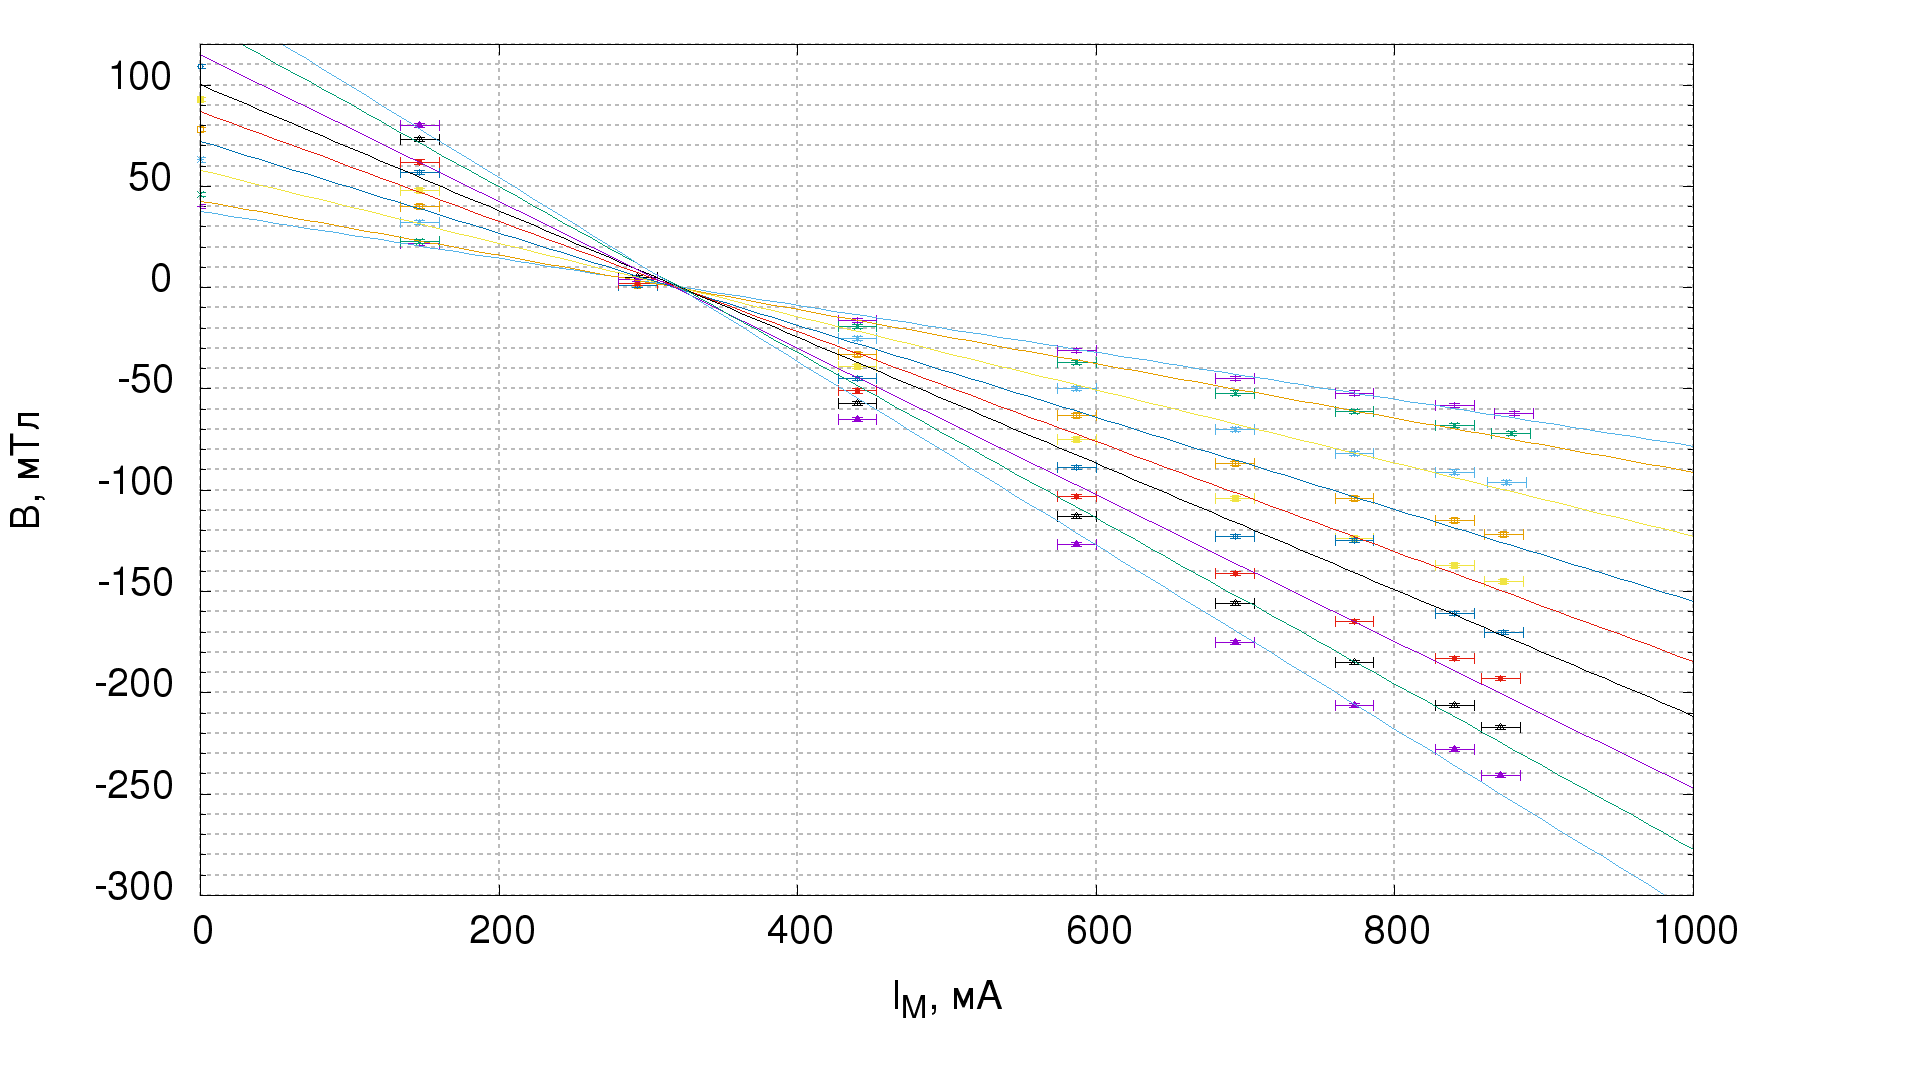
\includegraphics[width=0.99\textwidth]{data.png}
\end{center}
Построим график $k = f(I)$, рассчитаем угловой коэффициент и по формуле $U_{34} = -R_x \cdot \frac{IB}{a}$ рассчитаем постоянную Холла $R_X$.

\begin{center}
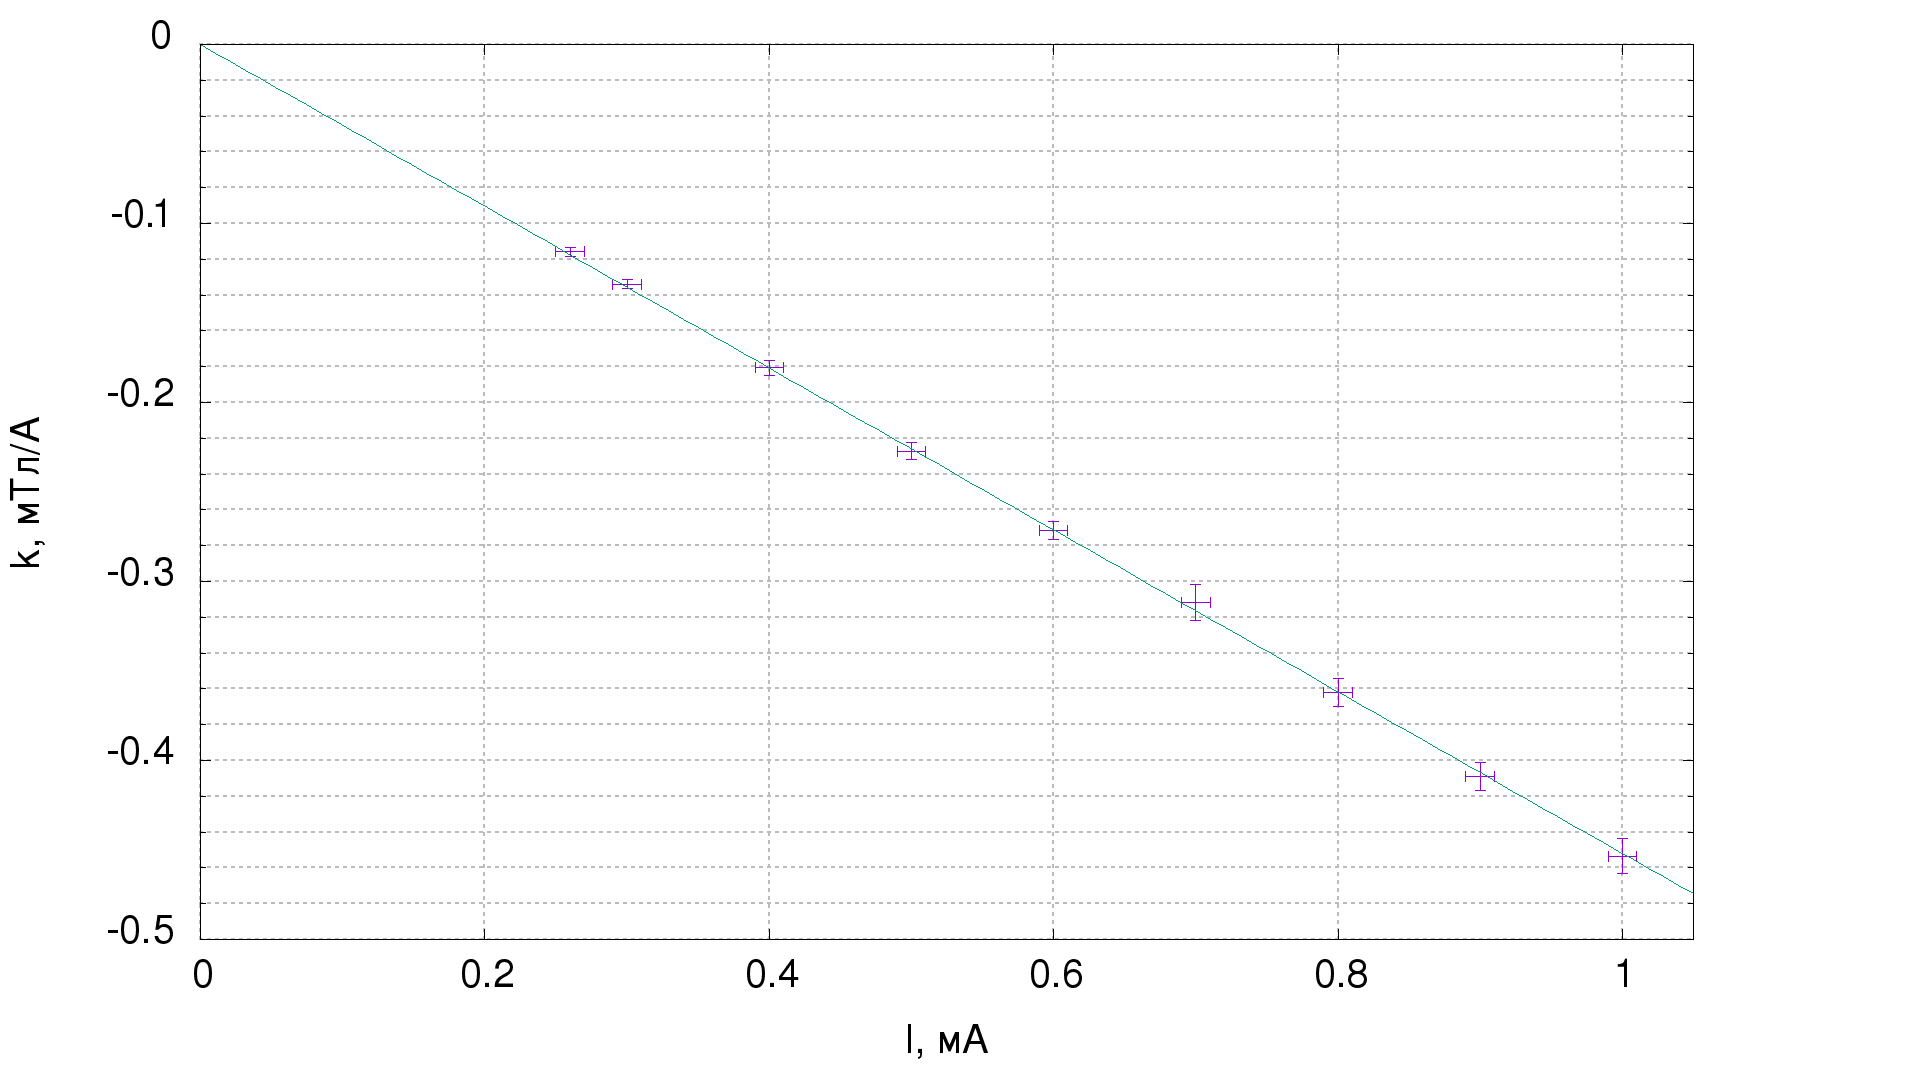
\includegraphics[width=0.99\textwidth]{sum.png}
\end{center}

\begin{center}
\begin{tabular}{|c|c|c|}\hline
$I\text{, \text{мА}}$&$k\text{, \text{мТл}/\text{А}}$&$\Delta k\text{, \text{мТл}/\text{А}}$\\\hline
$0.26$&$-0.115$&$0.003$\\\hline
$0.30$&$-0.133$&$0.003$\\\hline
$0.40$&$-0.180$&$0.004$\\\hline
$0.50$&$-0.227$&$0.005$\\\hline
$0.60$&$-0.271$&$0.005$\\\hline
$0.70$&$-0.31$&$0.01$\\\hline
$0.80$&$-0.361$&$0.008$\\\hline
$0.90$&$-0.408$&$0.008$\\\hline
$1.00$&$-0.45$&$0.01$\\\hline
\end{tabular}\\~\\
$\Delta I=0.01\,\text{\text{мА}}$
\end{center}


Из графика
$$\frac{Rx}{a} = (0.4519\pm0.0011) \frac{\text{м}^2}{\text{Кл}}.$$
В нашей установке $a=2.2\text{мм}.$
$$Rx = (0.994\pm0.002)\cdot10^{-3} \frac{\text{м}^3}{\text{Кл}}.$$

Определим, что наши частицы движутся к клемме 4 образца. Зная направление магнитного поля в электромагните и тока через образец, мы определяем, что наши частицы заряжены отрицательно, т.е. являются электронами.\\
Теперь определим концентрацию электронов:
$$n = \frac{1}{Rx\,e} = (6.28\pm0.01)\cdot 10^{21}\,\frac{1}{\text{м}^3}$$

По формуле $\sigma = \dfrac{IL_{35}}{U_{35}al}$ рассчитаем удельную проводимость материала образца для максимального тока $I = 1,00 \pm 0,02~\text{мА}$, напряжения $U_{35} = 552 \pm 1~\text{мкВ}$ и $L_{35} = 6.0~\text{мм}, a = 2.2~\text{мм}, l = 7~\text{мм}$:
$$\sigma = 706 \pm 15 \dfrac{1}{\text{Ом}\cdot\text{м}}$$
Подвижность электронов:
$$b = \frac{\sigma}{en} = (0.70\pm0.02)\frac{\text{м}^2}{\text{В}\cdot\text{с}}$$

\section*{Вывод}
Мы изучили явление эффекта Холла в полупроводниках, измерили для нашего образца (Германий) такие величины как постоянная Холла, концентрацию электронов, удельную проводимость и подвижность электронов.
\end{document}


125





\lipsum[1-4]
\begin{wrapfigure}{R}{5cm}
\centering
\includegraphics[width=0.20\textwidth]{rd.png}
\caption{1}
\end{wrapfigure}
\lipsum[1-6]


\begin{figure}[h]
\begin{center}$
\begin{array}{cccc}
\includegraphics[width=0.20\textwidth]{rd.png}&
\includegraphics[width=0.20\textwidth]{rd.png}&
\includegraphics[width=0.20\textwidth]{rd.png}&
\includegraphics[width=0.20\textwidth]{rd.png}\\
(1) & (2) & (3) & (4)
\end{array}$
\end{center}
\end{figure}
